\subsection{Rule based Head on}\label{s:testRuleHeadOn}

\paragraph{Scenario:} Two \emph{UAS} are going on same \emph{airway} in same \emph{flight level} in opposite direction in \emph{controlled airspace} (over 500 feet Above the Ground Level). The \emph{mutual position} of UAS can be classified as \emph{Side Approach}. Following \emph{collision hazard} is present:

\begin{enumerate}
    \item \emph{Head on Collision Hazard} - There is an \emph{UAS} approaching from opposite direction which invokes need to actively avoid \emph{Collision Point}.
\end{enumerate}
      
\noindent\emph{Head on Collision Hazard} must be addressed by \emph{UTM} service in the following manner:
    
\begin{enumerate}
    \item \emph{Each UAS} in particular \emph{Controlled Space} periodically sends synchronized \emph{Position Notification} messages (tab. \ref{tab:positionNotification}). 
    
    \item \emph{UTM} service receives \emph{Position Notifications} and manages \emph{Collision Cases} (tab. \ref{tab:collisionCase}) in \emph{Controlled Space}. 
    
    \item \emph{UTM} detects single \emph{Head on Collision Cases} with \emph{Collision Point} in  vicinity.
    
    \item \emph{UTM} service creates \emph{Virtual Roundabout} and implements \emph{Normative Directive} on both \emph{UAS}.
\end{enumerate}

\noindent\emph{Mission parameters} for four UAS systems are defined in (tab. \ref{tab:missionSetupRuleBasedHeadOnScenario}).

\begin{table}[H]
    \centering
    \begin{tabular}{c||c|c||c}
        \multirow{2}{*}{UAS} &\multicolumn{2}{c||}{Position} & \multirow{2}{*}{$\mathscr{WP}_1$} \\\cline{2-3}
          & $[x,y,z]$           & $[\theta,\varpi,\psi]$           & \\\hline\hline
        1 & $[0,20,0]^T $       & $[0^\circ,0^\circ,0^\circ]^T$    & $[45,20,0]^T$\\\hline 
        2 & $[40,20,0]^T $       & $[0^\circ,0^\circ,180^\circ]^T$    & $[-5,20,0]^T$\\
    \end{tabular}
    \caption{Mission setup for \emph{Rule based head on} scenario.}
    \label{tab:missionSetupRuleBasedHeadOnScenario}
\end{table}

\paragraph{Assumptions:} Following assumptions are valid for this test:
    
\begin{enumerate}
    \item \emph{Controlled Airspace Airworthiness} - UAS system is equipped with necessary controlled airspace equipment like ADS-B In/Out, Radar, Transponder, etc. Moreover airworthy \emph{UAS} has capability to precisely follow \emph{UTM directives} (max. 5 $\%$ deviation).
    
    \item \emph{C2 (Command \& control) Link Established} - necessary for (UAS $\leftrightarrow$ UAS) and (UAS $\leftrightarrow$ UTM) communication. If \emph{C2} link is lost the \emph{UAS} will enter into \emph{Emergency avoidance mode}.
    
    \item \emph{Decision frame synchronization with UTM} - necessary in discrete $C2$ environment otherwise \emph{safety margins} needs to be \emph{bloated}.
    
    \item \emph{Both UAS have identical cruising speed} - simplification impacting \emph{UTM} service implementation. \emph{Obstacle Avoidance Framework} can comprehend various intruders speed, with proper \emph{UAS} directives.
\end{enumerate}

\paragraph{Main Goal:} Show possibility of \emph{Head on situation resolution} with \emph{forced safety margin} by \emph{UAS Traffic Management} system.  The \emph{Obstacle Avoidance Framework based on Reach Sets} is used as \emph{Navigation Module}.


\paragraph{Acceptance  Criteria:} Following criteria must be met:

\begin{enumerate}
    \item \emph{Well Clear Condition valid for both UAS} - Both \emph{UAS} must have \emph{minimal required distance} from \emph{other UAS} for all \emph{Virtual Roundabout} enforcement time.
    
    \item \emph{Fulfillment of UTM Directives} - Both UAS must stay in \emph{Navigation mode} for all \emph{Virtual Roundabout} enforcement time. Both \emph{UAS} must stay on \emph{Virtual Roundabout} for necessary time, before leaving for \emph{Original Navigation waypoint $\mathscr{WP}_1$}.
\end{enumerate}

\paragraph{Testing Setup:} The \emph{standard test setup} for each UAS defined in (tab. \ref{tab:testMovementOrientations}, \ref{tab:testUASBasicParameters}, \ref{tab:testNavigationGridBasic}, \ref{tab:testAvoidanceGridBasic}, \ref{tab:testUASColoring}) is used with following parameter override:
\begin{enumerate}
    \item \emph{Navigation grid - type} - \emph{ACAS-like} with enabled \emph{Horizontal maneuvers}
\end{enumerate}

This \emph{configuration} is based on assumption that both UAS is in \emph{controlled airspace} in \emph{FL450} (flight level 45000 feet Above Sea Level), without permission for \emph{climb or descent maneuver}. \emph{Rule engine} is initialized in standard \emph{Rules of the air} configuration (fig. \ref{fig:RuleEngineInstanceLevels}).

There is \emph{UTM} service for given \emph{airspace cluster} calculating \emph{collision cases} (tab. \ref{tab:collisionCase}) based on incoming \emph{UAS position notifications} (tab. \ref{tab:positionNotification}).

\paragraph{Simulation Run:} Notable moments from the \emph{simulation run} (fig. \ref{fig:testCaseRuleBasedHeadOnApproach}) are following:

\begin{enumerate}
    \item\emph{Collision Case creation} (fig. \ref{fig:ruleBasedHeadOnSituationCollisionCaseCreation}) following events happens in this step:
    \begin{enumerate}[a.]
        \item Two UAS are on same airway approaching each other from opposite direction, UAS 1 (blue) from the left, UAS 2 (cyan) from the right.
        
        \item They are going to \emph{collide} at point $\mathscr{C}=[20,20,0]^T$ of \emph{Flight Level} (Elevation is 45, 000 feet Above Mean Sea Level).
        
        \item UTM service notices future \emph{Collision Situation} and creates \emph{Collision Case}.
        
        \item \emph{Virtual Roundabout} is created at \emph{collision point} with radius $10 m$. UTM issues directive for both UAS to avoid collision point from different sides.
        
        \item UAS 1 (blue) receives directive to avoid \emph{Collision Point} from \emph{right side} (Down side in GCS). UAS 2 (cyan) receives directive to avoid \emph{Collision Point} from \emph{right side} (Up side in GCS).

        \item Both UAS enters into \emph{Virtual Roundabout}.
    \end{enumerate}
    
    \item\emph{Well clear before} (fig. \ref{fig:ruleBasedHeadOnWellClearBefore}) UAS 1 (blue) is keeping \emph{enforced safety margin} (10 m) from \emph{collision point} and \emph{UAS 2 position}. The \emph{Virtual Roundabout} is enforced until the (\emph{Collision point}) is reached by both UAS. Both UAS stays in \emph{Navigation Mode}.
    
    \item\emph{Well clear after} (fig. \ref{fig:ruleBasedHeadOnWellClearAfter}) UTM notices that \emph{Collision point level} has been reached by both UAS. UTM renounce \emph{Directives} and enables a return to \emph{Original Waypoint} $\mathscr{WP}_1$. Both UAS starts to converging to \emph{Original waypoint} (because possible collision was averted).
    
    \item\emph{Waypoint reach} (fig. \ref{fig:ruleBasedHeadOnWaypointsReach}) Both UAS reaches respective goal points.
\end{enumerate}

\begin{figure}[H]
    \centering
    \begin{subfigure}{0.75\textwidth}
        \centering
        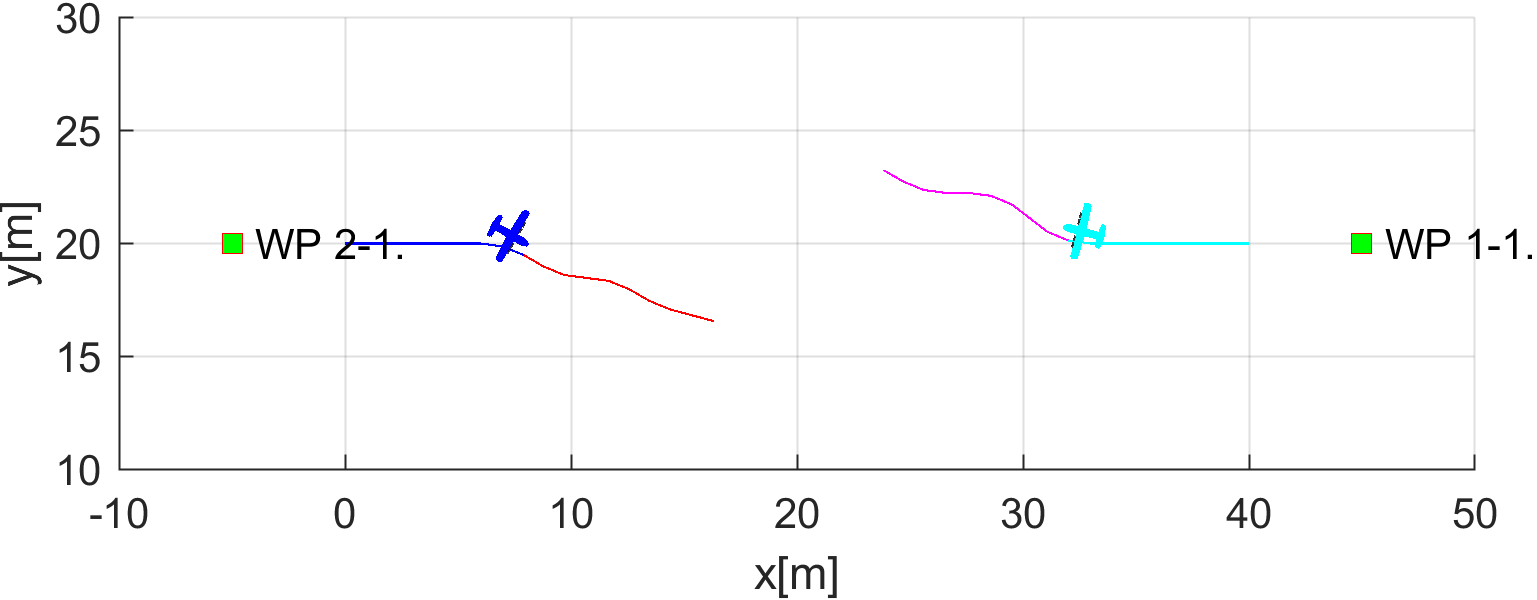
\includegraphics[width=0.9\linewidth]{\FIGDIR/NS055UtmCooperativeHeadOn00008}
        \caption{Collision case creation.}
        \label{fig:ruleBasedHeadOnSituationCollisionCaseCreation}
    \end{subfigure}
    \\
    \begin{subfigure}{0.75\textwidth}
        \centering
        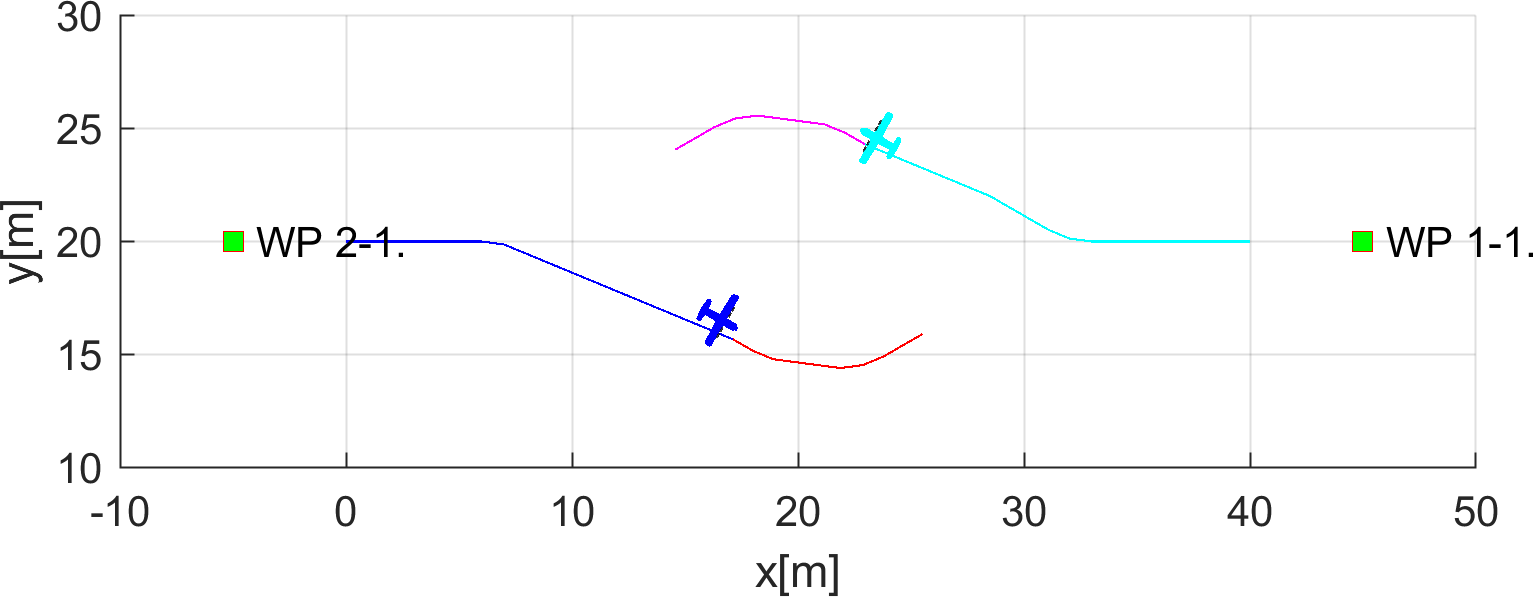
\includegraphics[width=0.9\linewidth]{\FIGDIR/NS056UtmCooperativeHeadOn00018} 
        \caption{Well clear before.}
        \label{fig:ruleBasedHeadOnWellClearBefore}
    \end{subfigure}
    \\
    \begin{subfigure}{0.75\textwidth}
        \centering
        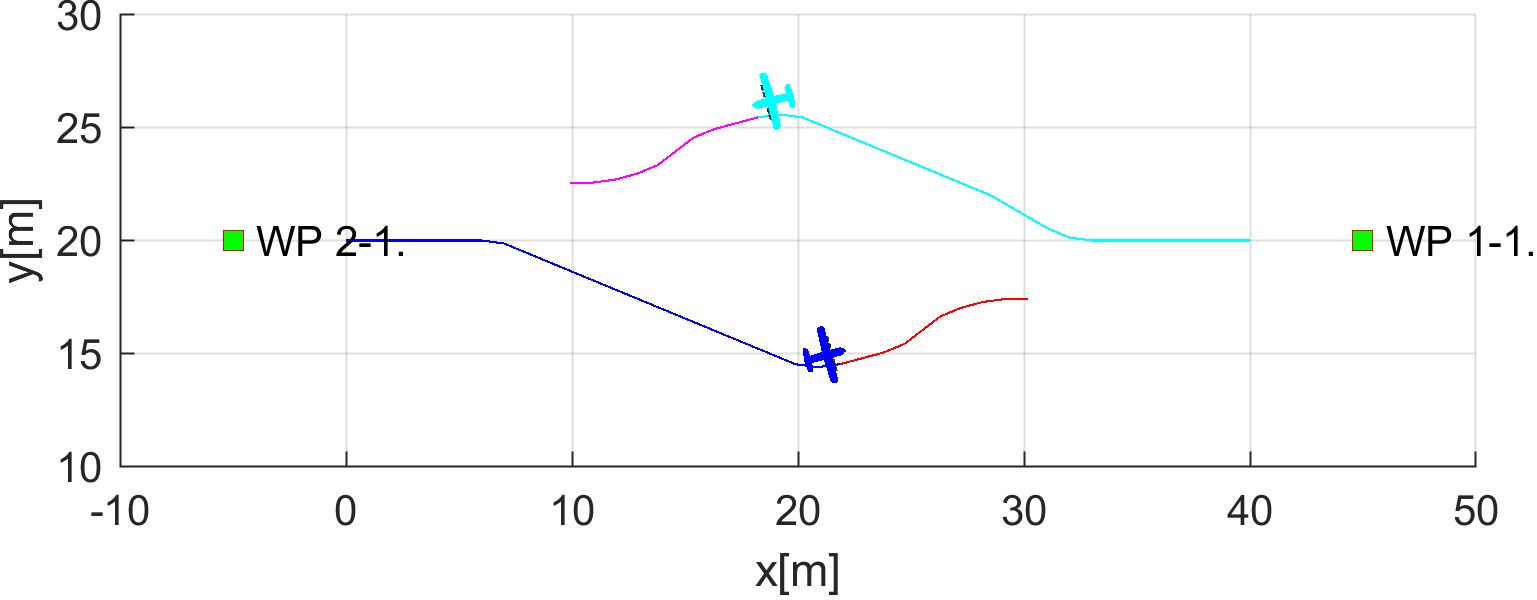
\includegraphics[width=0.9\linewidth]{\FIGDIR/NS057UtmCooperativeHeadOn00023} 
        \caption{Well clear after.}
        \label{fig:ruleBasedHeadOnWellClearAfter}
    \end{subfigure}
    \\
    \begin{subfigure}{0.75\textwidth}
        \centering
        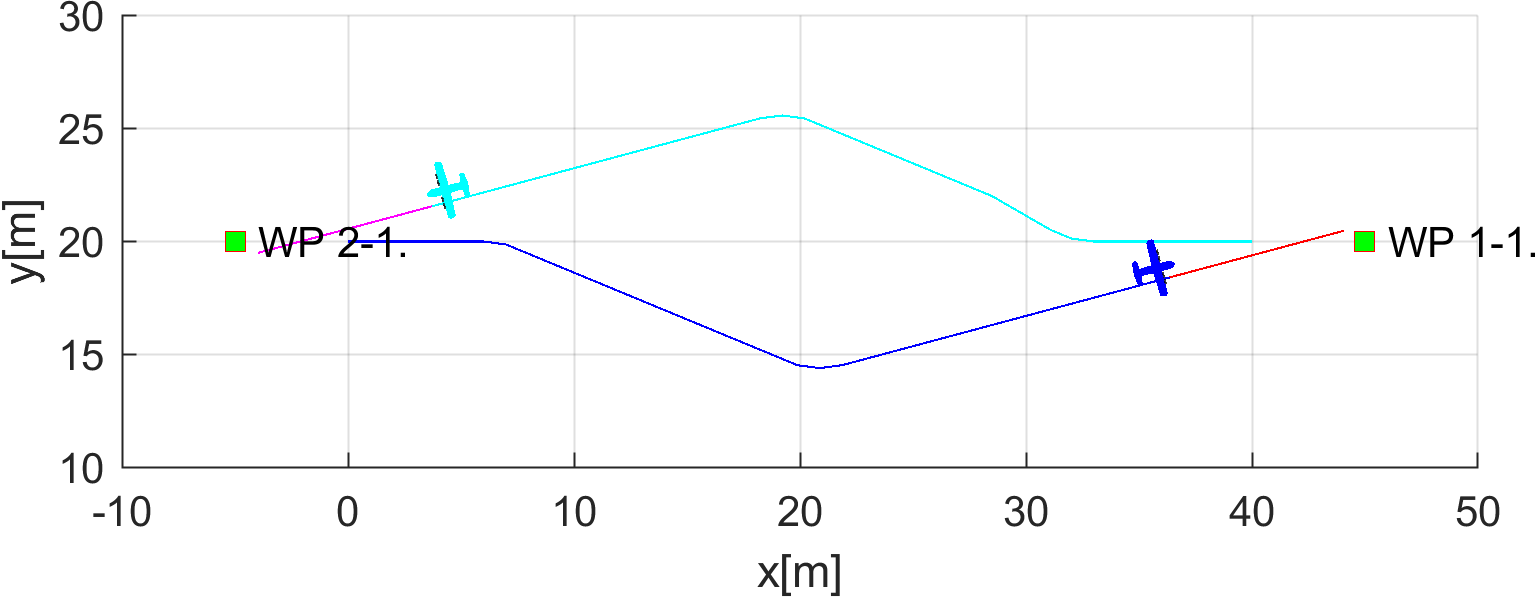
\includegraphics[width=0.9\linewidth]{\FIGDIR/NS058UtmCooperativeHeadOn00038} 
        \caption{Waypoints reach.}
        \label{fig:ruleBasedHeadOnWaypointsReach}
    \end{subfigure}
    \caption{Test scenario for \emph{Rule based head on approach} (virtual roundabout). }
    \label{fig:testCaseRuleBasedHeadOnApproach}
\end{figure}

\paragraph{Collision Case Calculation: } For test scenario in (fig. \ref{fig:testCaseRuleBasedHeadOnApproach}) where UAS 1 (blue) have head on collision with UAS 2 (cyan), \emph{Collision Case} have been calculated (tab. \ref{tab:collisionCasesRuleBasedHeadon}).

The \emph{Collision point} is at $[20,20,0]^T$ in Flight Level $FL450$ coordinate frame.

The \emph{angle of approach} was evaluated as $180^{\circ}$ which indicates \emph{Head on Approach} due the $130^\circ \le angle of Approach \le 180^\circ$ condition.

The \emph{mutual position} of UAS 1 (blue) and UAS 2 (cyan) is giving the roles of \emph{Roundabout} to \emph{both} UAS.

The \emph{safety margin} for \emph{Well Clear} was determined as $5m$ for UAS 1 and UAS 2. The combined \emph{Case Margin} is 10 m, which is sum of both. The \emph{mutual distance} can not go below this threshold.


\begin{table}[H]
    \centering
    \begin{tabular}{c|c|c|c|c|c||c|c}
        \multicolumn{6}{c||}{Collision Case}& \multicolumn{2}{c}{Margins} \\ \hline
        id  & UAS & role & \begin{tabular}[c]{@{}c@{}}collision\\ point\end{tabular} & \begin{tabular}[c]{@{}c@{}}angle of\\ approach\end{tabular} & type&  safety  & case  \\ \hline\hline
        % Case 1-2
        \multirow{2}{*}{1-2} & 1   & Roundabout & \multirow{2}{*}{$[20,20,0]^T$} & \multirow{2}{*}{$180^\circ$} & \multirow{2}{*}{Head on} & 5 & \multirow{2}{*}{10} \\ \cline{2-3} \cline{7-7} & 2   & Roundabout & & & & 5 & 
    \end{tabular}
    \caption{Collision case for \emph{Rule-based head on} scenario.}
    \label{tab:collisionCasesRuleBasedHeadon}
\end{table}

\paragraph{Safety Margin Performance:} The safety margin(well clear) (fig. \ref{fig:testCaseRuleBasedHeadOnAvoidancePerformance}) in controlled airspace are much rather than in non-controlled airspace (near miss) (fig. \ref{fig:testCaseHeadOnAvoidancePerformance}).

The enforced rule war (rule \ref{tab:ruleHeadonApproach}) with parameters: Collision Point $[20,20,0]^T$ and \emph{Safety Margin} $10m$ as given by Collision Case (tab. \ref{tab:collisionCasesRuleBasedHeadon}).

The mutual \emph{UAS} distance (blue line) does not go over \emph{Safety Margin} (red line) which means  both UAS well clear margins are not broken by any means (fig. \ref{fig:testCaseRuleBasedHeadOnApproach}).


\begin{figure}[H]
    \centering
    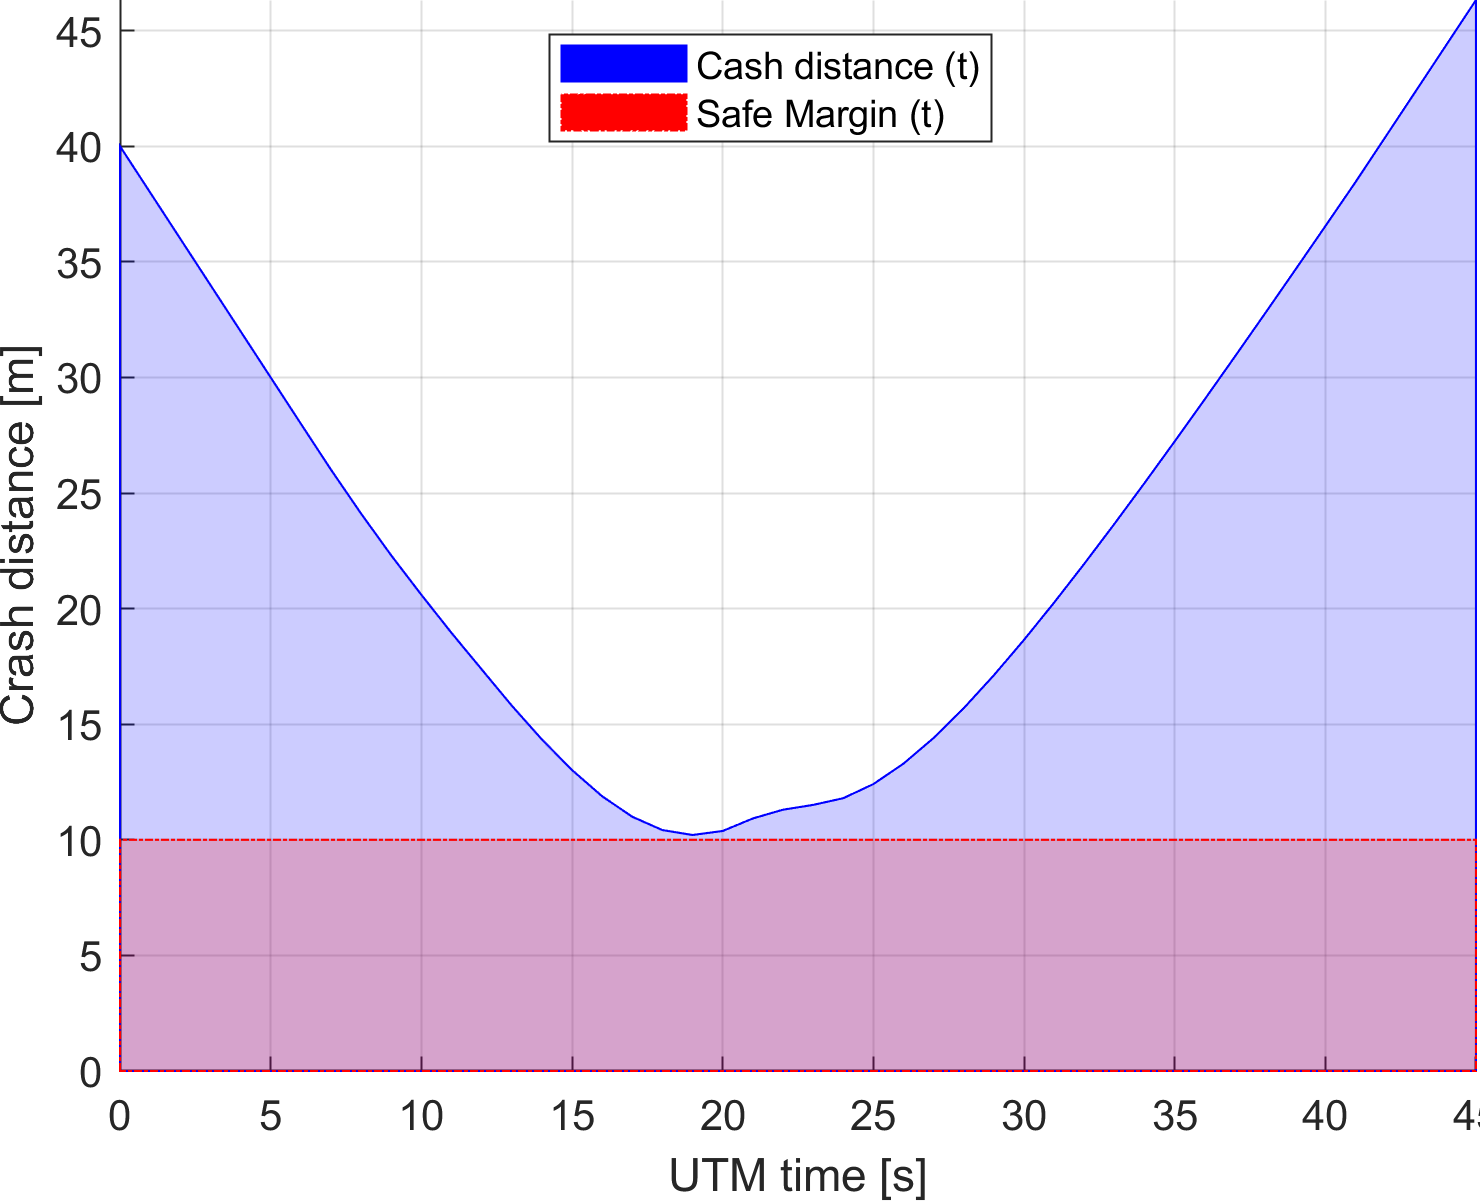
\includegraphics[width=0.55\linewidth]{\FIGDIR/NS059UtmCooperativeHeadOnPerformance} 
    \caption{\emph{Rule based head on} safety margin performance.}
    \label{fig:testCaseRuleBasedHeadOnAvoidancePerformance}
\end{figure}


\paragraph{Safety Margin Distance} (tab. \ref{tab:testCaseRuleBasedHeadOnSafetyMarginDistances}) represents the proximity on UAS mutual distance to breach \emph{well clear condition}. The \emph{well clear breach condition} was achieved. The \emph{minimal safety margin distance} was $0.2084 m$. The \emph{maximal safety margin distance} was $36.3253 m$ which represents distance at \emph{Collision Case} closing. 

\begin{table}[H]
    \centering
    \begin{tabular}{c||c|c|c}
        \multirow{2}{*}{UAS:} & \multicolumn{3}{c}{Safety margin distance} \\ \cline{2-4} 
                  & min          & max         & breach         \\ \hline\hline
            1-2   & 0.2084       & 36.3253     & false          \\ 
    \end{tabular}
    \caption{\emph{Rule based head on} safety margin distances.}
    \label{tab:testCaseRuleBasedHeadOnSafetyMarginDistances}
\end{table}

\paragraph{Path Tracking Performance:} \emph{Path tracking} is displayed in (fig. \ref{fig:ruleBasedHeadOnTrajectoryTrackingPerformance}). The \emph{UAS} trajectory is divined into \emph{X, Y, Z axis tracking over UTM Time}. The \emph{Reference Trajectory} (green dashed line) interconnect starting position of UAS (green square marked S) an goal waypoint (green square marked 1). The \emph{Executed Trajectory} (blue solid line) reflects real UAS trajectory. 

\begin{enumerate}
    \item UAS 1. (fig, \ref{fig:ruleBasedHeadOnUAS1PathTracking}) do steady right side \emph{roundabout maneuver} (y-axis).
    
    \item UAS 2. (fig. \ref{fig:ruleBasedHeadOnUAS2PathTracking}) do steady right side \emph{roundabout maneuver} (y-axis).
\end{enumerate}

\begin{figure}[H]
	\centering
    \begin{subfigure}{0.48\textwidth}
    	\centering
        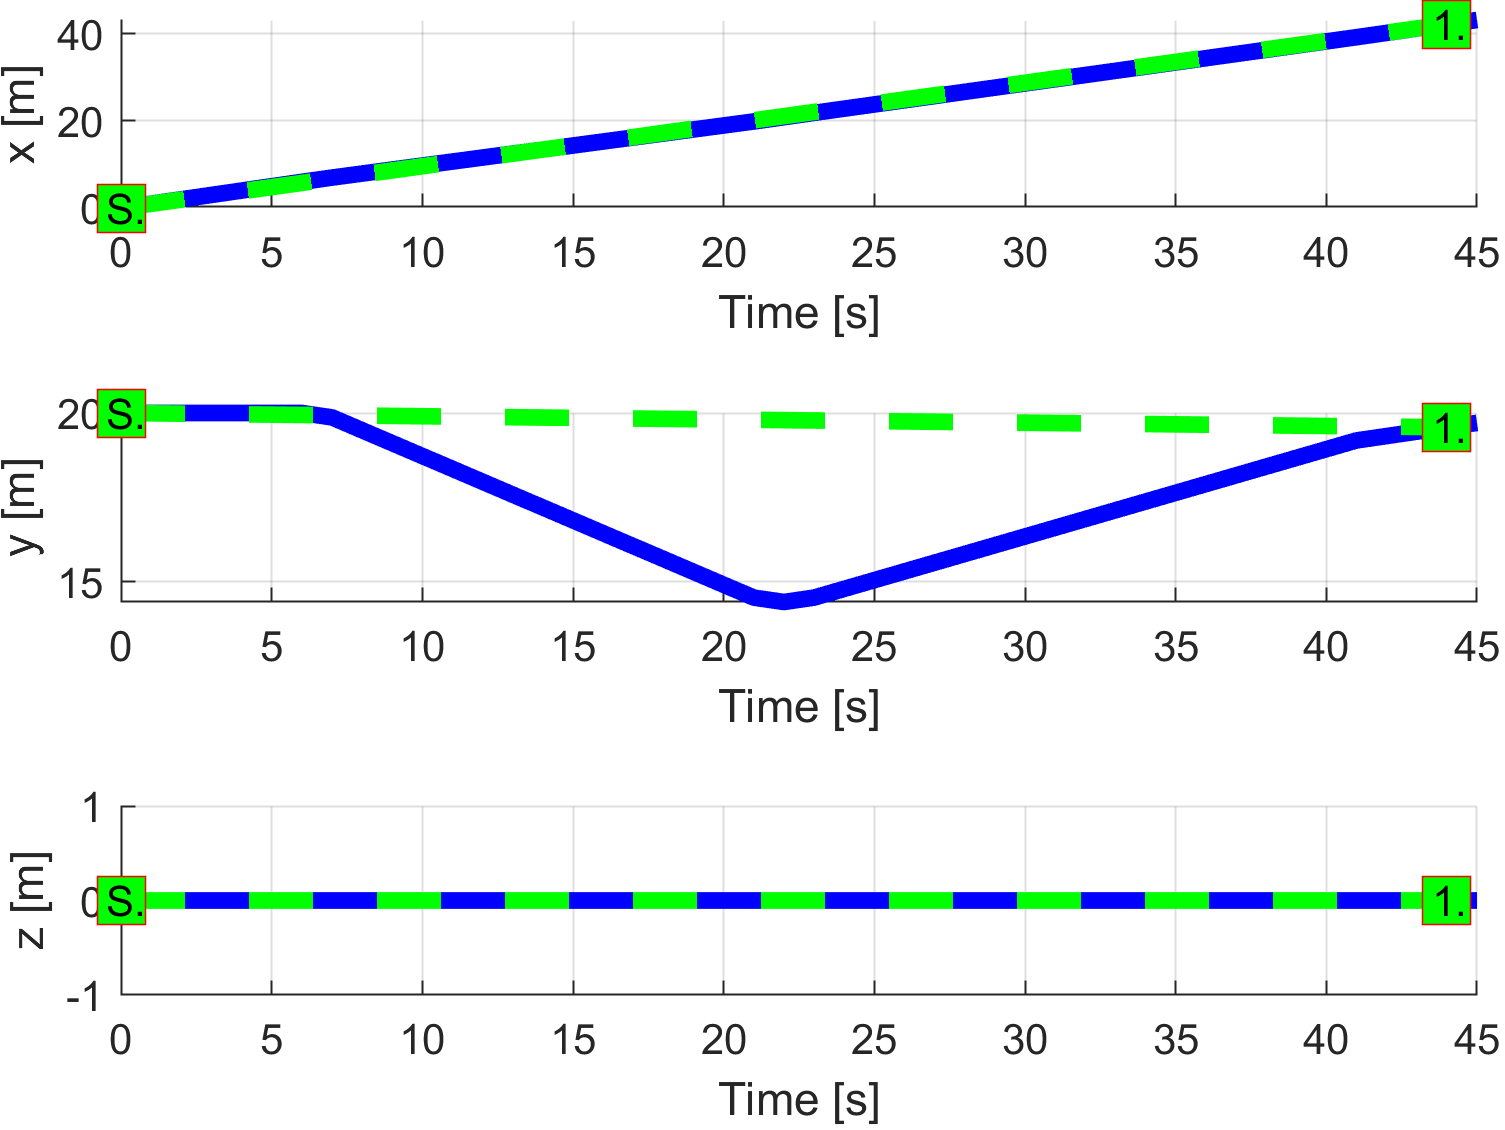
\includegraphics[width=0.9\linewidth]{\FIGDIR/NS060UtmCooperativeHeadOnUAV1PathFollowing}
        \caption{UAS 1.}
        \label{fig:ruleBasedHeadOnUAS1PathTracking}
    \end{subfigure}
    \begin{subfigure}{0.48\textwidth}
    	\centering
        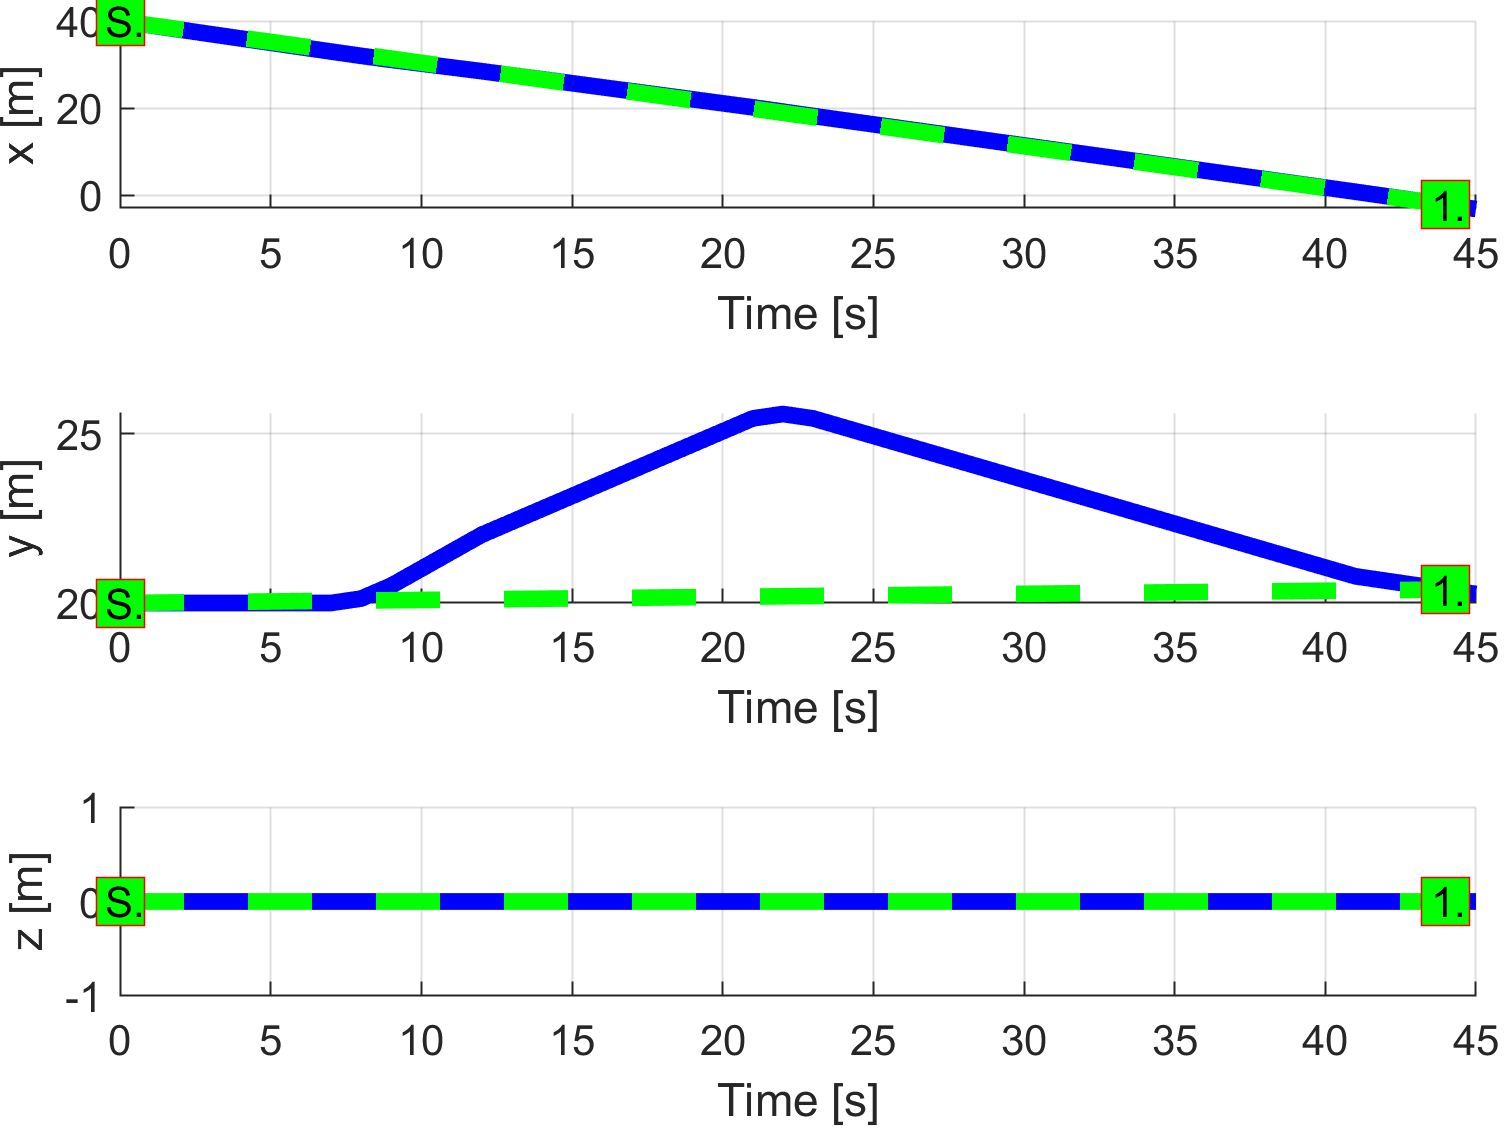
\includegraphics[width=0.9\linewidth]{\FIGDIR/NS061UtmCooperativeHeadOnUAV2PathFollowing} 
        \caption{UAS 2.}
        \label{fig:ruleBasedHeadOnUAS2PathTracking}
    \end{subfigure}
    \caption{\emph{Trajectory tracking} for \emph{Rule based head on} test case. }
    \label{fig:ruleBasedHeadOnTrajectoryTrackingPerformance}
\end{figure}

\paragraph{Path Tracking Deviations:} Deviations (tab. \ref{tab:pathTrackingParametersForRuleBasedHeadOn}) are in \emph{expected ranges}, considering the \emph{mission plans} (tab. \ref{tab:missionSetupRuleBasedHeadOnScenario}) and \emph{Collision Case} safety margin of $10 m$.

\begin{table}[H]
    \centering
    \begin{tabular}{c||c|c}
        \multirow{2}{*}{Param.} & UAS 1     & UAS 2              \\\cline{2-3}
                        & $\mathscr{WP}_1$  & $\mathscr{WP}_1$   \\\hline\hline
          $\max |x|$    & 0                 & 0                  \\\hline
          $\max |y|$    & 5.40              & 5.40              \\\hline
          $\max |z|$    & 0                 & 0                  \\\hline
          $\max dist.$  & 5.40              & 5.40              \\
    \end{tabular}
    \caption{Path tracking properties for \emph{Rule based head on} scenario.}
    \label{tab:pathTrackingParametersForRuleBasedHeadOn}
\end{table}